\documentclass[10pt]{article}
\usepackage[margin=1in]{geometry}
\usepackage{amsmath,amsfonts,amsthm,amssymb,amsopn}
\usepackage{graphicx}

\def\E{\mathbb{E}}
\def\N{\mathcal{N}}
\def\I{\mathbb{I}}
\def\Var{\text{Var}}

\newtheorem{theorem}{Theorem}
\graphicspath{figs/}

\begin{document}
\title{CM229: Homework 1}
\author{Nick Mancuso}
\maketitle

\begin{enumerate}
\item
\begin{enumerate}
\item
Let $N_x = \sum_i^n x_i$ denote the number of ``successes'' observed. We can write the
likelihood of $p$ as \[ \mathcal{L}(p| X) = {n \choose N_x} p^{N_x} (1 - p)^{n - N_x}.\] In order
to find the ML-estimate of the likelihood we perform the equivalent operation of maximizing the
log-likelihood, defined as \[\ell(p | X) = N_x \log p + (n - N_x) \log (1 - p) + O(1),\] whose
derivative is given by, \[ \frac{d \ell}{d p} = \frac{N_x}{p} - \frac{n - N_x}{1 - p}.\] Setting
equal to 0 and solving we see,
\begin{align*}
    \frac{N_x - pn}{p(1 - p)} = 0 \Leftrightarrow 
    \frac{N_x}{n} = p \Leftrightarrow 
    \hat{p} = \frac{\sum_i^n x_i}{n}.
\end{align*}

\item
The second derivative of the log-likelihood is given as, 
\[ \frac{d^2 \ell}{d p^2} = \frac{-N_x}{p^2} - \frac{n - N_x}{(1 - p)^2}.\] Therefore, we can
compute the Fisher Information as
\begin{align*}
    I_n(p) = -\E\left[\frac{-N_x}{p^2} - \frac{n - N_x}{(1 - p)^2} \middle\rvert p \right] = 
    \E\left[\frac{N_x}{p^2} + \frac{n - N_x}{(1 - p)^2} \middle\rvert p \right]
    &= \E\left[\frac{N_x}{p^2} \middle\rvert p\right] + \E\left[\frac{n - N_x}{(1 - p)^2} \middle\rvert p \right] \\
    &= \frac{n p}{p^2} + \frac{n (1 - p)}{(1 - p)^2}\\
    &= \frac{n}{p} + \frac{n}{1 - p} \\
    &= \frac{n}{p(1 - p)}.
\end{align*}
\item
The distribution of $\hat{p}$ is asymptotically Normal with mean $p$ and var $\frac{p(1 - p)}{n}$.
\item
\item
\item
\end{enumerate}

\item
\begin{enumerate}
\item
\item
\item
\end{enumerate}

\item
\begin{enumerate}
\item
The second derivative of $f(x)$ is given by, \[\frac{d^2 f}{d x^2} = -\frac{1}{x^2}.\] This new function
is negative at all points other than 0, hence $f$ is concave.
\item
The second derivative of $f(x)$, \[\frac{d^2 f}{d x^2} = \frac{\exp(x)(1 - \exp(x))}{(1 +
\exp(x))^3}.\] For values $x \leq 0$ then $f(x)$ will be non-negative; however, when $x > 0$
$f(x)$ will be negative due to the $1 - \exp(x)$ term. Thus $f$ is neither concave nor convex.
\end{enumerate}

\item
\begin{enumerate}
\item
The RSS can be written as norm of a linear function, which is the composition of two convex
functions and hence is convex. However we will show more directly by second-order conditions.
We define RSS using vector/matrix notation as, \[RSS(\beta) = (y - X\beta)^t(y - X\beta)\] whose
second derivative is given by,
\begin{align*}
    \frac{\partial RSS^2}{\partial \beta \partial \beta} = 2X^t X.
\end{align*}
Now, RSS is convex iff $x^tX^tXx \geq 0$ for any $x \in \mathbb{R}^n$. Let $Xx \triangleq u$, then
$x^tX^tXx = u^t u = \sum_i u_i^2 \geq 0,$ hence RSS is convex. Another ``proof'' can be given by 
looking at the eigenvalues of $X^tX$. If the SVD of $X$ is $U^t\Sigma V$, then 
\[
    X^tX = (U^t\Sigma V)^t (U^t\Sigma V) = V^t\Sigma U U^t\Sigma V = V^t \Sigma \Sigma V = V^t \Sigma^2 V.
\] Note that this is a valid eigendecomposition whose eigenvalues are the diagonal elements of
$\Sigma^2$, each of which $\sigma^2_i \geq 0$, thus $X^tX$ is positive semidefinite, and hence RSS is convex.

\item
All the expectations are conditional on $X$, however I've dropped them for notational simplicity.
\begin{align*}
    \text{bias}(\hat{\beta}) &= \E[\hat{\beta} - \beta] = \E[(X^tX)^{-1}X^ty - \beta] = \E[(X^tX)^{-1}X^t(X\beta - \varepsilon)] - \beta \\
    &= (X^tX)^{-1}X^tX\beta - (X^tX)^{-1}X^t\E[\varepsilon] - \beta = \beta - 0 - \beta  = 0.
\end{align*}
Before performing our variance calculations first note from our above calclations that
$\hat{\beta} - \beta = (X^tX)^{-1}X^t \varepsilon.$ Now we can compute variance of our estimator
$\hat{\beta}$ as,
\begin{align*}
    \Var(\hat{\beta}) & = \Var(\hat{\beta} - \beta) = \Var((X^tX)^{-1}X^t \varepsilon) \\
    & = (X^tX)^{-1}X^t \Var(\varepsilon) ((X^tX)^{-1}X^t)^t =  (X^tX)^{-1}X^t \E(\varepsilon \varepsilon^t) ((X^tX)^{-1}X^t)^t \\
    & = (X^tX)^{-1}X^t \sigma^2 I_n ((X^tX)^{-1}X^t)^t  = \sigma^2(X^tX)^{-1}
\end{align*}
\item
Bias and variance for the predicted value $\hat{y}_*$ can be comptued by,
\begin{align*}
    \text{bias}(\hat{y}_*) &= \E[\hat{y}_* - y] = \E[\hat{\beta}^t x_*] - \E[y] = \E[\hat{\beta}^t]x_* - \E[\beta^t x_* - \varepsilon] \\
    &= \E[\hat{\beta}^t]x_* - \beta^t x_* - \E[\varepsilon] = \beta^t x_* - \beta^t x_* - 0 = 0
\end{align*} and
\[\Var(\hat{y}_*) = \Var(\hat{y}_* - y) = \Var(\varepsilon) = \sigma^2 (X^t X)^{-1}.\]
If we make the assumption that $\varepsilon_i \sim N(0, \sigma^2)$ then $\hat{y}_* \sim N(\hat{\beta}^t x_*, \sigma^2 (X^t X)^{-1}).$

\item
The log-likelihood can be written as $\ell(\theta | X) \propto (y - X\beta)^t W^{-1} (y - X\beta)$
where $W = \text{diag}(w_1, \dotsc, w_n)$ The MLE is given by solving for the root at the first derivative
\[
    \frac{\partial \ell}{\partial \theta} = - 2 X^t W^{-1}(y - X\beta) \Leftrightarrow 
    X^tW^{-1}X\beta = X^t W^{-1}y \Leftrightarrow \hat{\beta} = (X^t W^{-1} X)^{-1} X^t W^{-1} y
 \]
\end{enumerate}


\item
\begin{enumerate}
\item
We can reject the null for (1-based indexing) phenotype 2 at SNP 258 ($p=1.13\text{E-92}$), phenotype
3 at SNP 119 ($p=4.7\text{E-7}$) and phenotype 4 at SNP 43 ($p=1.08\text{E-8}$).
\item

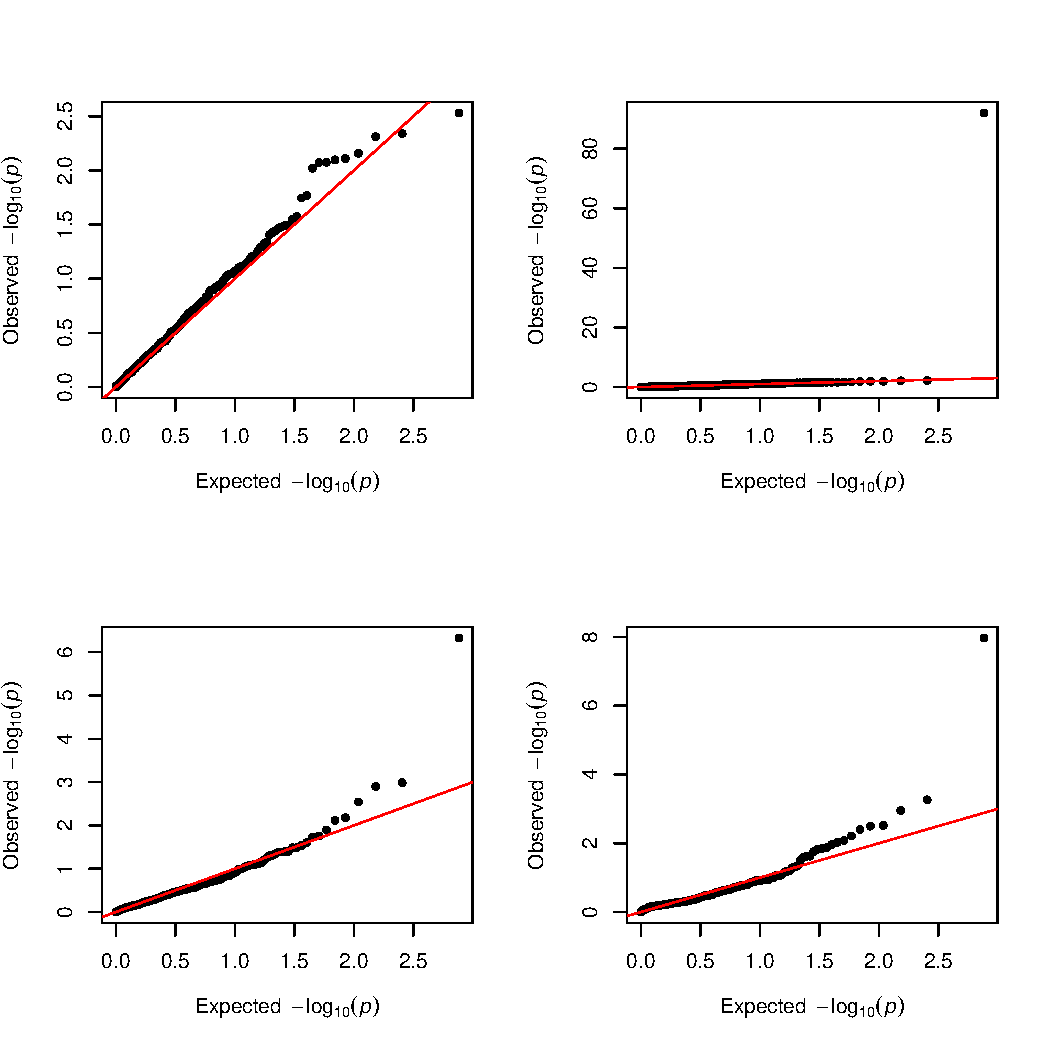
\includegraphics[width=0.75\textwidth]{figs/qqplot.pdf}

\item
\item
An alternative test for significance is to perform permutation tests where we permute phenotypes
across individuals. This should, in theory, break association between genotype and phenotype. If 
we observe the strength of association to lay in the tails of this empirical distribution we can
be somewhat more confident that our association is not spurious. There are however, other
confounding factors that could arise (Ancestry, batch effects, etc.).
\end{enumerate}
\end{enumerate}
\end{document}
